\usepackage[utf8]{inputenc}
\usepackage[T1]{fontenc}
\usepackage{mathptmx}
\usepackage[scaled=.90]{helvet}
\usepackage{courier}
\usepackage{caption}
\captionsetup{labelformat=empty,labelsep=none}
\usepackage{verbatim}
\usepackage{hyperref}
\usepackage{listings}
% strikethrough (\sout)
\usepackage{ulem}
\lstset{language=Perl,basicstyle=\normalsize,tabsize=3,showstringspaces=false}

\newcommand {\framedgraphic}[2] {
    \begin{frame}{#1}
        \begin{center}
            \includegraphics[width=\textwidth,height=0.8\textheight,keepaspectratio]{#2}
        \end{center}
    \end{frame}
}

\setbeamerfont{single}{size=\Huge}
\setbeamerfont{double}{size=\LARGE}

\title{TableEditor}
\author[racke]{Stefan Hornburg (Racke)\\ \texttt{racke@linuxia.de}}
\date{17. Deutscher Perl-Workshop, Dresden, 7. Mai 2015}

\begin{document}
\maketitle{}

\begin{frame}
  \titlepage
\end{frame}

\tableofcontents

% \section{Übersicht}

% DBIx::Class ist mit Sicherheit einer der größten Schätze von "Modern Perl"
% und bietet schnelle und komfortable Datenbankabfragen.

% Ebenso erleichtert Dancer das Erstellen von Webanwendungen mit einer leicht
% verständlichen Programmierung.

% Wie können beide zusammen genutzt werden? Zunächst mit dem DBIC Plugin für
% Dancer. Mit diesem können mehrere DBIx::Class Schemas innerhalb der
% Dancer-Anwendung verwenden werden.

% Um auch die Dancer-Sessions in der Datenbank zu speichern, habe ich eine Engine für Dancer und DBIC geschrieben.

% Außerdem werde ich ein Projekt vorstellen, mit dem man einfach den Inhalt
% von Datenbanken mittels eines DBIx::Class Schemas editieren kann.

% \begin{frame}<handout:0>{Übersicht}
% \begin{itemize}
% \item Einführung
% \item DBIC Schemas mit Dancer Plugin
% \item DBIC session engine
% \item Tabelleneditor
% \end{itemize}
% \end{frame}

% Wir starten mit einer kurzen Einführung von DBIx::Class.
\begin{frame}{}
\begin{center}
\usebeamerfont{single}
CGI.pm must die ...
\end{center}
\end{frame}

\begin{frame}{}
\begin{center}
\usebeamerfont{single}
... and we bury DBI alive!
\end{center}
\end{frame}

\begin{frame}{}
\begin{center}
\usebeamerfont{single}
Dancer und DBIx::Class
\end{center}
\end{frame}

\section{Anwendungen}
\begin{frame}{}
\begin{center}
\usebeamerfont{single}
Anwendungen
\end{center}
\end{frame}

% \begin{frame}{Datenbank}
% \begin{itemize}
% \item Datenbank
% \item Tabellen
% \item Datensätze
% \end{itemize}
% \end{frame}

% \begin{frame}{DBIx::Class}
% \begin{itemize}
% \item Schema
% \item ResultSet
% \item Row / Objekt
% \end{itemize}
% \end{frame}

\subsection{Interchange6}
\begin{frame}{eCommerce Software}
\begin{itemize}
\item \sout{Magento}
\item Interchange6
\end{itemize}
\end{frame}

\subsection{TableEditor}
\begin{frame}{Datenbankadministration}
\begin{itemize}
\item \sout{phpmyadmin}
\item \sout{phppgadmin}
\item TableEditor
\end{itemize}
\end{frame}

\begin{frame}{TableEditor Features}
\begin{itemize}
\item Unterstützung mehrerer Datenbanksysteme \\
      MySQL, PostgreSQL, ...
\item höherer Abstraktionslevel
\item modernes Frontend
\item wenig Quellcode
\item ``einfache'' Installation
\end{itemize}
\end{frame}

Der TableEditor hat ein modernes Frontend. Es basiert
auf den Javascript-Paketen Bootstrap und Angular.
Die Templates und ein Teil der Logik sind somit Teil
des Frontends.

% \begin{frame}{Anmeldung}
%   \begin{center}
%     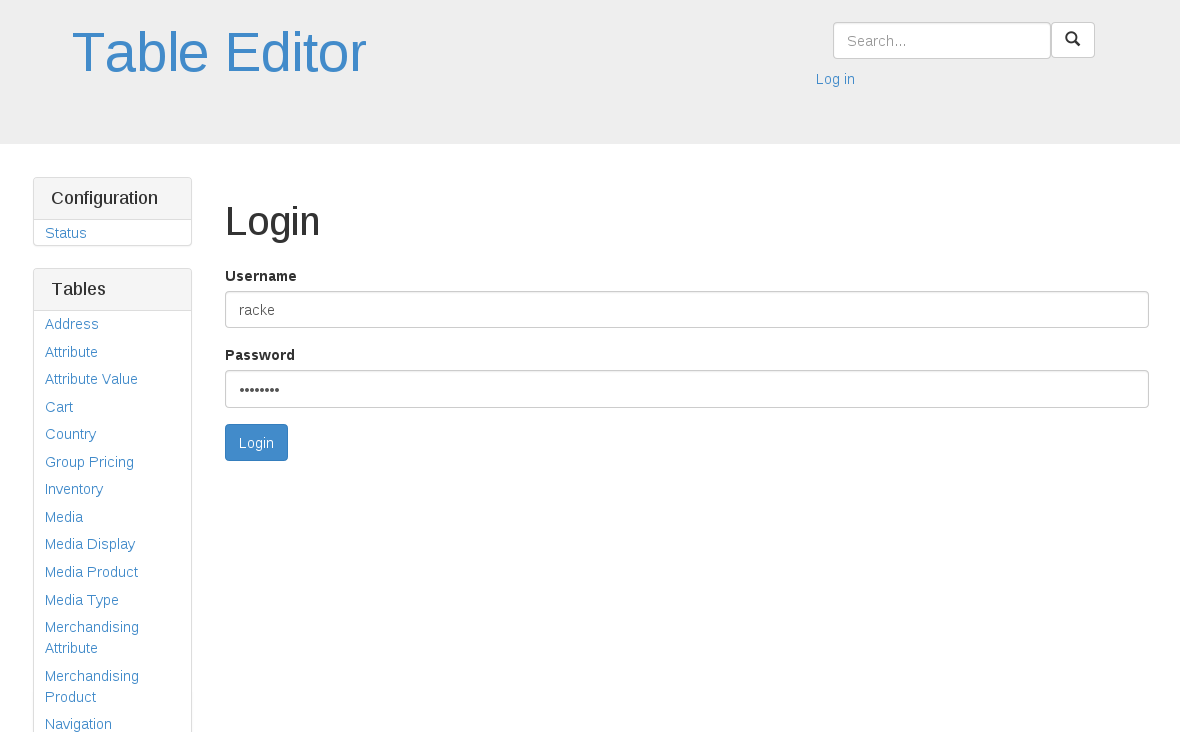
\includegraphics[width=\textwidth,height=0.8\textheight,keepaspectratio]{images/login.png}
%   \end{center}
% \end{frame}

\begin{frame}{Eingabe Datenbankparameter}
  \begin{center}
    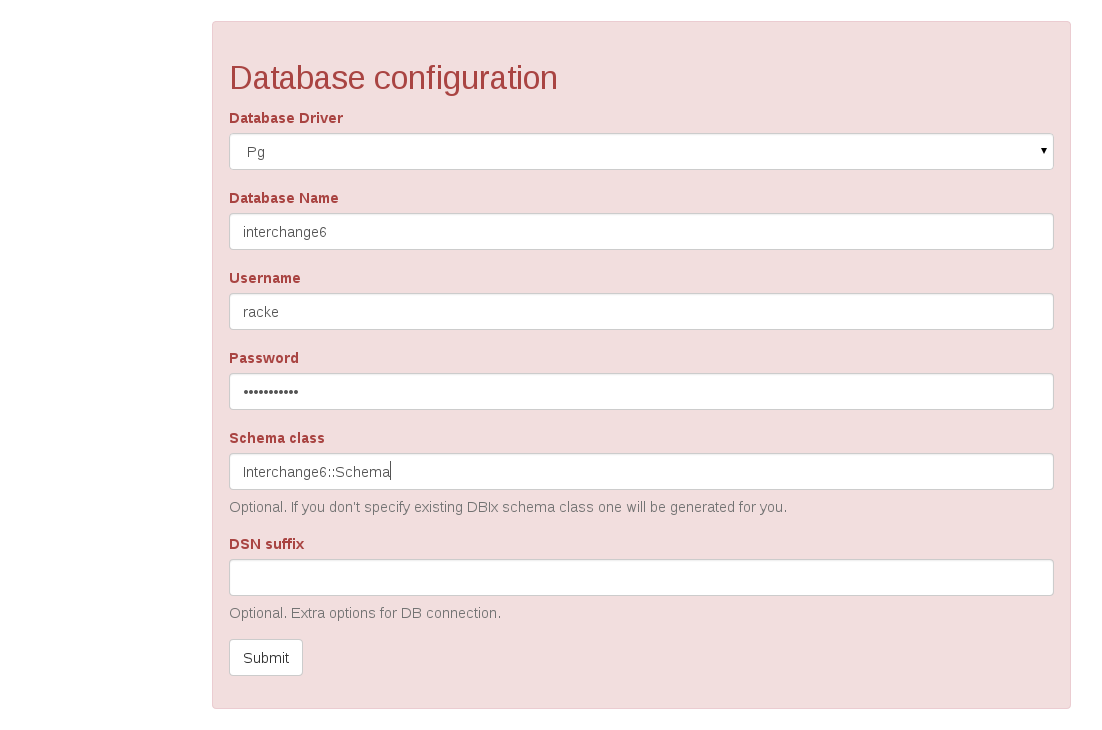
\includegraphics[width=\textwidth,height=0.8\textheight,keepaspectratio]{images/input.png}
  \end{center}
\end{frame}

\begin{frame}{Ansicht Produkte}
  \begin{center}
    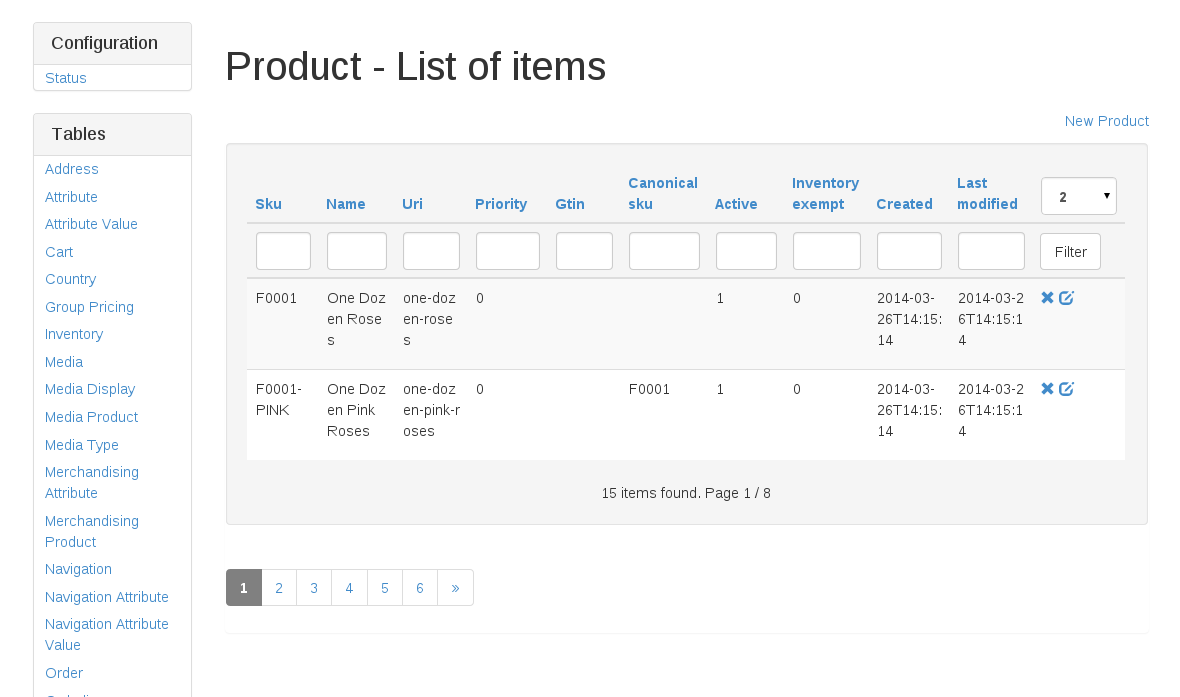
\includegraphics[width=\textwidth,height=0.8\textheight,keepaspectratio]{images/product.png}
  \end{center}
\end{frame}

\begin{frame}{Ansicht Produkt}
  \begin{center}
    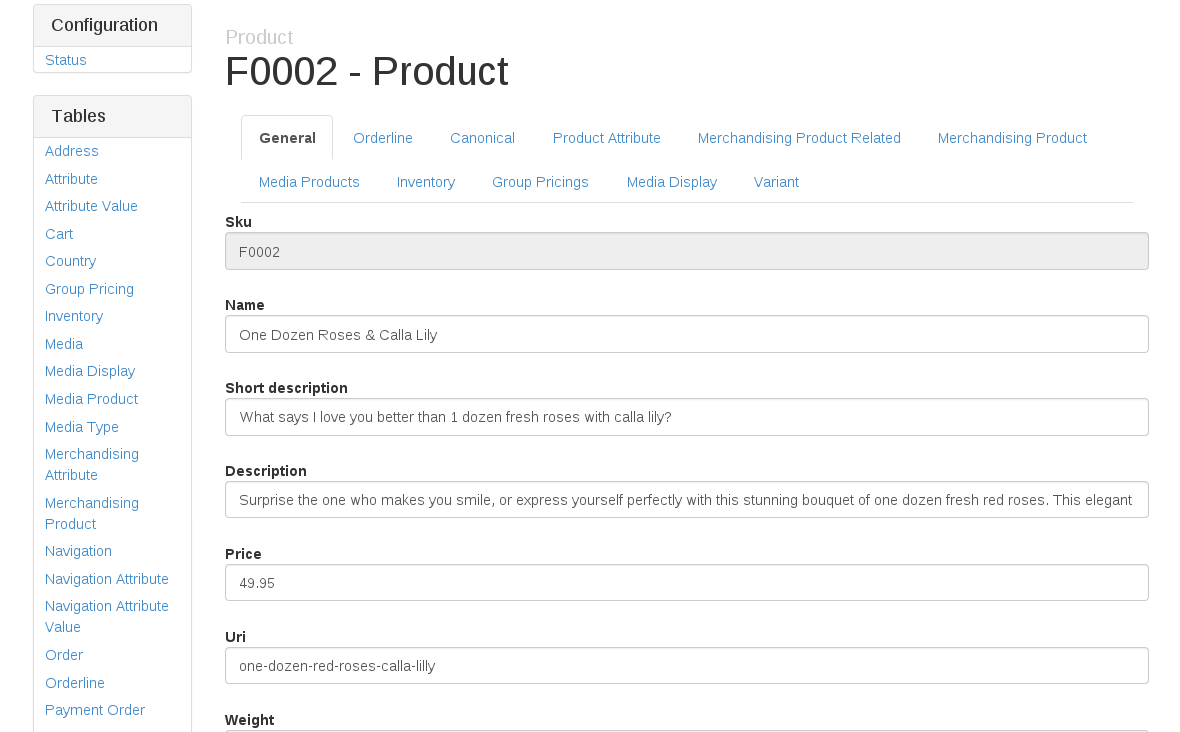
\includegraphics[width=\textwidth,height=0.8\textheight,keepaspectratio]{images/product-detail.png}
  \end{center}
\end{frame}

\begin{frame}{Beziehung Orderline}
  \begin{center}
    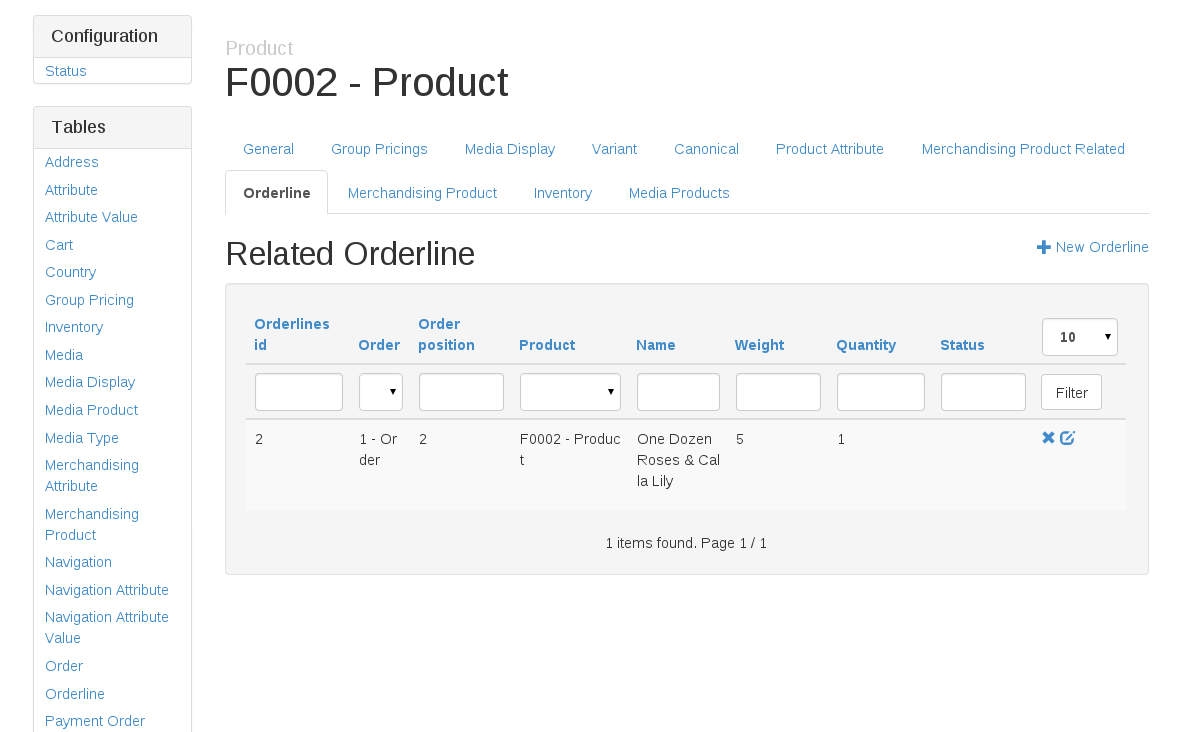
\includegraphics[width=\textwidth,height=0.8\textheight,keepaspectratio]{images/product-related.png}
  \end{center}
\end{frame}

% \subsection{Dropbox}
% \begin{frame}{Dropbox}
% \begin{itemize}
% \item \href{https://github.com/melmothx/dancer-plugin-dropbox}{Dropbox Plugin}
% \end{itemize}
% \end{frame}

\section{Dancer::Plugin::DBIC}

\begin{frame}{Übersicht Dancer::Plugin::DBIC}
\begin{itemize}
\item Anwendung
\item Konfiguration
\item UTF-8
\item Schema erzeugen
\end{itemize}
\end{frame}

\subsection{Anwendung}
\begin{frame}[fragile]{DBIx::Class ohne Dancer Plugin}
\begin{lstlisting}
use Interchange6::Schema;

$schema = Interchange6::Schema->connect(...);

$schema->resultset('User')->search({..});
\end{lstlisting}
\end{frame}

\begin{frame}[fragile]{DBIx::Class mit Dancer Plugin}
\begin{lstlisting}
use Dancer::Plugin::DBIC;

schema->resultset('User')->search({..});

resultset('User')->search({..});

rset('User')->search({..});
\end{lstlisting}
\end{frame}

\subsection{Konfiguration}

Im Normalfall verwendet man nur ein Schema in seiner
Dancer-Anwendung:

\begin{frame}[fragile]{Konfiguration}
\begin{lstlisting}
plugins:
  DBIC:
    default:
      dsn: dbi:mysql:interchange6
      user: racke
      pass: nevairbe
      schema_class: Interchange6::Schema
\end{lstlisting}
\end{frame}

Es sind aber auch mehrere möglich:

\begin{frame}[fragile]{Mehrere Schemas}
\begin{lstlisting}
plugins:
  DBIC:
    default:
      dsn: dbi:mysql:interchange6
      user: racke
      pass: nevairbe
      schema_class: Interchange6::Schema
    legacy:
      dsn: dbi:mysql:interchange5
      user: racke
      pass: nevairbe
      schema_class: Interchange5::Schema
\end{lstlisting}
\end{frame}

Das Schema \verb|legacy| wird dann wie folgt verwendet:

\begin{frame}[fragile]{Mehrere Schemas}
\begin{lstlisting}
use Dancer::Plugin::DBIC;

schema('legacy')->resultset('UserDb')->search({..});
\end{lstlisting}
\end{frame}

\subsection{UTF-8}
Im Gegensatz zu Dancer::Plugin::Database bietet das DBIC-Plugin
keine automatische Unterstützung für UTF-8. Also ist die entsprechende
DBI-Option in der Konfiguration einzutragen, hier für MySQL:
\begin{frame}[fragile]{UTF-8 für MySQL}
\begin{lstlisting}
plugins:
  DBIC:
    default:
      dsn: dbi:mysql:interchange6
      user: racke
      pass: nevairbe
      schema_class: Interchange6::Schema
      options:
        mysql_enable_utf8: 1
\end{lstlisting}
\end{frame}

Die Optionen für die gängigen Datenbanken in der Übersicht:

\begin{description}
\item[SQLite] \verb|sqlite_unicode: 1|
\item[MySQL] \verb|mysql_enable_utf8: 1|
\item[PostgreSQL] \verb|pg_enable_utf8: 1| 
\end{description}

\subsection{Schema dynamisch erzeugen}
Das DBIC-Plugin erzeugt dynamisch ein DBIx::Class::Schema, wenn
die Schema-Klasse (\verb|schema_class|) nicht angegeben wird.
Dazu ist das Modul DBIx::Class::Schema::Loader erforderlich.

Dies ist nicht empfehlenswert für den Produktionseinsatz, jedoch
praktisch für den Tabelleneditor.

\begin{frame}[fragile]{Schema dynamisch erzeugen}
\begin{itemize}
\item \verb|schema_class| fehlt in Konfiguration
\item DBIx::Class::Schema::Loader
\item Test und Entwicklung
\item TableEditor
\end{itemize}
\end{frame}

\section{TableEditor}

\begin{frame}<handout:0>{Übersicht TableEditor}
\begin{itemize}
\item Installation
\item Frontend
\item Routes
\item Anmeldung
\item Beziehungen
\item Einschränkungen
\item Konfiguration
\end{itemize}
\end{frame}

\subsection{Installation}
Im günstigsten Fall kann die Installation mit 4 Schritten
erledigt werden:

\begin{frame}[fragile]{Installation}
\begin{lstlisting}
git clone https://github.com/interchange/TableEditor
cd TableEditor
cpanm .
./bin/app.pl
\end{lstlisting}
\end{frame}

\begin{frame}[fragile]{Driver}
\begin{itemize}
\item DBD::mysql
\item DBD::Pg
\item ...
\end{itemize}
\end{frame}

\subsection{Frontend}
Das Frontend für den TableEditor ist mit Angular und Bootstrap erstellt.
Das Theme kann sehr einfach durch Austausch der CSS-Datei für Bootstrap
geändert werden.

\begin{frame}<handout:0>{Frontend}
\begin{itemize}
\item Angular
\begin{itemize}
\item Routes für das Frontend
\item XHR-Abfragen an REST API
\item JSON
\end{itemize}
\item Bootstrap
\item Theme
\end{itemize}
\end{frame}

\subsection{Routes}
\begin{frame}[fragile]{Routes}
\begin{lstlisting}
get '/:class/:id' => require_login sub {
    # retrieve database record and add relationships
    ...

    return to_json($data, {allow_unknown => 1});
};
\end{lstlisting}
\end{frame}

\subsection{Anmeldung}

Für die Integration von Authentifizierung in eine Dancer-Anwendung empfehlen
wir wärmestens das
\href{https://metacpan.org/pod/Dancer::Plugin::Auth::Extensible}{Auth::Extensible}
Plugin.

\begin{frame}{Anmeldung}
\begin{itemize}
\item Dancer::Plugin::Auth::Extensible
\item Provider
\begin{itemize}
\item Unix
\item DBIC
\end{itemize}
\item Datenbank \textit{(geplant)}
\end{itemize}
\end{frame}

\subsection{Beziehungen}

Beziehungen werden automatisch angezeigt.

\begin{frame}{Beziehungen}
\begin{itemize}
\item might\_have
\item has\_many
\item belongs\_to
\item many\_to\_many
\end{itemize}
\end{frame}

Filter

Es fehlen Felder in related orderline (Übersicht)

Different DBIC keys

Paging

\subsection{Einschränkungen}
\begin{frame}{Einschränkungen}
\begin{itemize}
\item Primärschlüssel für \textbf{eine} Spalte
\item Geschwindigkeit (komplexe Schemas)
\item Fehlerbehandlung
\end{itemize}
\end{frame}

\subsection{Konfiguration}
\begin{frame}{Konfiguration}
\begin{itemize}
\item Auth::Extensible
\item DBIC
% \begin{itemize}
% \item \verb|default|
% \end{itemize}
\end{itemize}
\end{frame}

\begin{frame}{Weitere Features}
\begin{itemize}
\item Suche (Solr)
\item Auswahl Schema
\end{itemize}
\end{frame}

\section{Ausblick und Mitarbeit}

\subsection{Entwicklung}

Das Git-Repository für den TableEditor befindet sich auf Github:

\begin{frame}{Entwicklung}
\url{https://github.com/interchange/TableEditor}
\end{frame}

\subsection{Dancer2}

Was ist mit Dancer2 ?

Für Dancer2 existiert bereits ein Plugin:

\url{https://metacpan.org/pod/Dancer2::Plugin::DBIC}

Die Sessionengine und der TableEditor wurden noch nicht auf Dancer2 portiert.

\begin{frame}{Dancer2}
  \begin{description}
  \item[Plugin::DBIC] \url{https://metacpan.org/pod/Dancer2::Plugin::DBIC}
  \item[Session::DBIC] noch nicht portiert
  \item[TableEditor] noch nicht portiert
  \end{description}
\end{frame}

% \section{Testing}
% DBIC, Plugin
% Testdatabase

\subsection{Slides}

\begin{frame}{Slides}
Slides:
\url{http://www.linuxia.de/talks/pws2014/dancer-dbic-de-beamer.pdf}
\end{frame}

\end{document}

%%% Local Variables: 
%%% mode: latex
%%% TeX-master: t
%%% End: 
